\documentclass[../Notes.tex]{subfiles}
\usepackage{../Style/Diagrams}
\usepackage{../Style/Master}
\usepackage{../Style/boxes}
\usepackage{../Style/DefNoteFact}
\usepackage{../Style/QnsProof}
\usepackage{../Style/Thms}
\usepackage{../Style/Env}
\usepackage{../Style/NewCommands}
\begin{document}
\chapter{Linear Algebra}
\begin{definition}{}{}
    A vector space (or linear space) \(V\) over a field \(\mathbb{F}\) consists of a set on which two operations (called addition and multiplication respectively here) are defined so that;
\begin{itemize}[label=(M1),leftmargin=*]
    \item[(A)](\(V\) is Closed Under Addition) For all \(\mathbf{x},\mathbf{y} \in V\), there exists a unique element \(\mathbf{x}+\mathbf{y} \in V\).
    \item[(M)](\(V\) is Closed Under Scalar Multiplication) For all elements \(a \in \mathbb{F}\) and elements \(\mathbf{x} \in V\), there exists a unique element \(a\mathbf{x} \in V\).
\end{itemize}
Such that the following properties hold:  
\begin{enumerate}[label=(VS {{\arabic*}}), leftmargin=*]
    \item \label{(VS 1)}(Commutativity of Addition) For all \(\mathbf{x},\mathbf{y} \in V\), we have \(\mathbf{x}+\mathbf{y}=\mathbf{y}+\mathbf{x}\).
    \item \label{(VS 2)}(Associativity of Addition) For all \(\mathbf{x},\mathbf{y},\mathbf{z} \in V\), we have \((\mathbf{x}+\mathbf{y})+\mathbf{z}=\mathbf{x}+(\mathbf{y}+\mathbf{z})\).
    \item \label{(VS 3)}(Existance of The Zero/Null Vector) There exists an element in \(V\) denoted by \({\mathbf{0}}\), such that \(\mathbf{x}+{\mathbf{0}}=\mathbf{x}\) for all \(\mathbf{x} \in V\).
    \item \label{(VS 4)}(Existance of Additive Inverses) For all elements \(\mathbf{x} \in V\), there exists an element \(\mathbf{y} \in V\) such that \(\mathbf{x}+\mathbf{y}={\mathbf{0}}\).
    \item \label{(VS 5)}(Multiplicative Identity) For all elements \(x \in V\), we have \(1\mathbf{x}=\mathbf{x}\), where 1 denotes the multiplicative identity in \(\mathbb{F}\).
    \item \label{(VS 6)}(Compatibility of Scalar Multiplication with Field Multiplication) For all elements \(a,b \in \mathbb{F}\) and elements \(\mathbf{x} \in V\), we have \((ab)\mathbf{x}=a(b\mathbf{x})\).
    \item \label{(VS 7)}(Distributivity of Scalar Multiplication over Vector Addition) For all elements \(a \in \mathbb{F}\) and elements \(\mathbf{x},\mathbf{y} \in V\), we have \(a(\mathbf{x}+\mathbf{y})=a\mathbf{x}+a\mathbf{y}\).
    \item \label{(VS 8)}(Distributivity of Scalar Multiplication over Field Addition) For all elements \(a,b \in \mathbb{F}\), and elements \(\mathbf{x} \in V\), we have \((a+b)\mathbf{x}=a\mathbf{x}+b\mathbf{x}\).
\end{enumerate}
\end{definition}
\begin{theorem}{}{}
    Let \(V\) be a vector space and \(W\) a subset of \(V\). Then \(W\) is a subspace of \(V\) iff the following 3 conditions hold for the operations defined in V.
            \begin{enumerate}[label=(\alph*)]
                \item \(\mathbf{0} \in W\) \label{Theorem 1.3(a)}
                \item \(\mathbf{x}+\mathbf{y} \in W\) whenever \(\mathbf{x} \in W\) and \(\mathbf{y} \in W\). \label{Theorem 1.3(b)}
                \item \(c\mathbf{x} \in W\) whenever \(c \in \mathbb{F}\) and \(\mathbf{x} \in W\). \label{Theorem 1.3(c)}
            \end{enumerate}
\end{theorem}
\begin{definition}{}{}
    A subset \(S\) of a vector space \(V\) \emph{generates} (or \emph{spans}) \(V\) iff \(\Span(S)=V\). In this case, we also say that the vectors of \(S\) generate (or span) \(V\).
\end{definition}
\begin{definition}{}{}
    Let \(V\) be a vector space and \(S\) a nonempty subset of \(V\). A vector \(v \in V\) is called a \emph{linear combination} of vectors of \(S\) iff there exists a finite number of vectors \(u_1,u_2,\dots,u_n\) in \(S\) and scalars \(a_1,a_2,\dots,a_n\) in \(\mathbb{F}\) such that
            \[v=\sum_{i=1}^{n}{a_iu_i}.\]
            In this case we also say that \(v\) is a linear combination of \(u_1,u_2,\dots,u_n\) and call \(a_1,a_2,\dots,a_n\) the \emph{coefficients} of the linear combination
\end{definition}
\begin{definition}{}{}
    A set subset \(S\) of a vector space \(V\) is called \emph{linearly dependent} iff there exists a finite number of distinct vectors \(u_1,u_2,\dots,u_n\)in \(S\) and scalars \(a_1,a_2,\dots,a_n\) not all zero, such that
            \[a_1u_1+a_2u_2+a_nu_n=\mathbf{0}.\]
\end{definition}
\begin{definition}{}{}
    A \emph{basis} \(\beta\) for a vector space \(V\) is a linearly independent subset of \(V\) that generates \(V\). If \(\beta\) is a basis for \(V\), we also say that the vectors of \(\beta\) form a basis for \(V\).
\end{definition}
\begin{theorem}{The Rank-Nullity Theorem.}{}
    For any vector spaces \(V\) and \(W\), and a linear operator \(T \colon V \to W\), it holds that
    \[\rank(T)+\nullity(T)=\dim(V).\]
\end{theorem}
\begin{stbox}{General Information}
    \begin{itemize}
        \item Let \(\mathbf{A}\) be an \(m\times n\) matrix, and \(\mathbf{a}_j\) its \(j\)th column. For any \(\mathbf{x}=
        \begin{pmatrix}
            x_1 & x_2 & \cdots & x_n\\
        \end{pmatrix}^\top\), 
        \[\mathbf{A}\mathbf{x}=\sum_{j=1}^{n}{x_j}\mathbf{a}_j.\]
        \item Let \(\mathbf{A}\) and \(\mathbf{B}\) be matrices having \(n\) rows. For any matrix \(\mathbf{M}\) with \(n\) columns, we have
        \[\begin{pNiceArray}{c|c}
            \mathbf{A} & \mathbf{B}
        \end{pNiceArray}=
        \begin{pNiceArray}{c|c}
            \mathbf{M}\mathbf{A} & \mathbf{M}\mathbf{B}
        \end{pNiceArray}.\]
    \end{itemize}
\end{stbox}
\begin{definition}{}{}
    A system \(\mathbf{A}\mathbf{x}=\mathbf{b}\) is \emph{homogeneous} iff \(\mathbf{b}=0\); otherwise it is \emph{nonhomogeneous}.
\end{definition}
\begin{theorem}{}{}
    For any matrix, its row space, column space, and rank are identical.
\end{theorem}
\begin{theorem}{}{}
    A system \(\mathbf{A}\mathbf{x}=\mathbf{b}\) of \(m\) linear equations in \(n\) unknowns has a solution space of dimension \(n-\rank(A)\).
\end{theorem}
\begin{definition}{}{}
    A system \(\mathbf{A}\mathbf{x}=\mathbf{b}\) of linear equations is \emph{consistent} iff its solution set is nonempty; otherwise it is \emph{inconsistent}.
\end{definition}
\begin{theorem}{The Rouché-Capelli Theorem.}{}
    A system \(\mathbf{A}\mathbf{x}=\mathbf{b}\) is consistent iff \(\rank(\mathbf{A})=\rank(\mathbf{A}\vert \mathbf{b})\).
\end{theorem}
\begin{definition}{}{}
    A matrix is said to be in \emph{reduced row echelon form} iff
        \begin{itemize}
            \item Any row containing a nonzero entry precedes any row in which all the entries are zero (if any).
            \item The first nonzero entry in each row is the only nonzero entry in its column.
            \item The first nonzero entry in each row is 1 and it occurs in a column to the right of the first nonzero entry in the preceding row.
        \end{itemize}
\end{definition}
\begin{stbox}{}
    \begin{itemize}
        \item Gaussian elimination. 
        \begin{itemize}
            \item In the forward pass, the augmented matrix is transformed into an upper triangular matrix in which the first nonzero entry of each row is 1 and it occurs in a column to the right of the first nonzero entry
            of each preceding row.
            \item  In the backward pass, the upper triangular matrix is transformed into reduced row echelon form by making the first nonzero entry of each row the only nonzero entry of its column.
        \end{itemize}
        \item Gaussian elimination always reduecs a matrix to its rref form.
        \item Let \(\mathbf{A}\) be an invertible \(n\times n\) matrix. Then, for some elementary row matrices \(\mathbf{E}_1\) to \(\mathbf{E}_p\),
        \[\mathbf{E}_p\mathbf{E}_{p-1}\dots \mathbf{E}_1(\mathbf{A} \,\vert\, \mathbf{I}_n)=\mathbf{A}^{-1}(\mathbf{A} \,\vert\, \mathbf{I}_n)=(\mathbf{I}_n \,\vert\, \mathbf{A}^{-1}).\]
        In other words, we can perform Gaussian elimination, so that \((\mathbf{A} \,\vert\, \mathbf{I}_n)\to (\mathbf{I}_n \,\vert\, \mathbf{A}^{-1})\).
        \item Let \(\mathbf{A}\coloneq
        \begin{pmatrix}
            \mathbf{a}_1&\mathbf{a}_2&\cdots&\mathbf{a}_n
        \end{pmatrix}\) be \(m\times n\) matrix, and \(\mathbf{A}'\coloneq
        \begin{pmatrix}
            \mathbf{a'}_1&\mathbf{a'}_2&\cdots&\mathbf{a'}_n
        \end{pmatrix}\) its rref. Then, \(\{\mathbf{a}_{k_1},\mathbf{a}_{k_2},\dots,\mathbf{a}_{k_m}\}\) is linearly independent iff \(\{\mathbf{a'}_{k_1},\mathbf{a'}_{k_2},\dots,\mathbf{a'}_{k_m}\}\) is. Moreover, the row space of \(\mathbf{A}\) and \(\mathbf{A}'\) are clearly identical.
        \item Finding a basis for an intersection of subspaces. Let \(V\) and \(W\) be subspaces of \(\mathbb{F}^n\) generated by the columns of the \(n\times m\) matrix \(\mathbf{A}\) and \(n\times k\) matrix \(\mathbf{B}\), respectively. Find a basis for the subspace \(V\cap W\). 
        \begin{enumerate}
            \item First notice that \(\mathbf{v} \in V\cap W\) iff
            \[\mathbf{v}=\mathbf{A}\mathbf{x}_1=\mathbf{B}\mathbf{x}_2\]
            for some \(\mathbf{x}_2\in \mathbb{F}^m\) and \(\mathbf{x}_2\in \mathbb{F}^k\). That is,
            \[\begin{pmatrix}
                \mathbf{A} & \mathbf{B} 
            \end{pmatrix}
            \begin{pmatrix}
                \mathbf{x_1}\\
                -\mathbf{x_2}
            \end{pmatrix}
            =\mathbf{0}.\]
            So, equivalently, we write
            \[\begin{pmatrix}
                \mathbf{A} & \mathbf{B} 
            \end{pmatrix}
            \mathbf{y}=\mathbf{0}.\]
            for some \(\mathbf{y}\in \mathbb{F}^{m+k}\). As such, by row reducing             
            \(\begin{pmatrix}
                \mathbf{A} & \mathbf{B} 
            \end{pmatrix}\), 
            we find a basis 
            \[\beta\coloneq\left\{
                \begin{pmatrix}
                    \mathbf{u_1}\\
                    \mathbf{u_1'}
                \end{pmatrix},
                \begin{pmatrix}
                    \mathbf{u_2}\\
                    \mathbf{u_2'}
                \end{pmatrix},\dots,
                \begin{pmatrix}
                    \mathbf{u_r}\\
                    \mathbf{u_r'}
                \end{pmatrix}
            \right\},\]
            where \(\mathbf{u}_i \in \mathbb{F}^m\) and \(\mathbf{u}_i \in \mathbb{F}^k\).
            Now, 
            % let \(\mathsf{u_i} \in \mathbb{F}^m\) be vector obtained by deleting all but the first \(m\) entries of \(\mathbf{u}_i\). Then,
            a generating set for \(V\cap W\) is
            \[\Gamma\coloneq\{\mathbf{A}\mathbf{u_1},\mathbf{A}\mathbf{u_2},\dots,\mathbf{A}\mathbf{u_r}\}.\]
            Alternatively, 
            % letting \(\mathsf{u'_i} \in \mathbb{F}^m\) be vector obtained by deleting all but the last \(k\) entries of \(\mathbf{u}_i\), 
            another generating set for \(V\cap W\) is
            \[\Delta\coloneq\left\{\mathbf{B}\mathbf{u'_1},\mathbf{B}\mathbf{u'_2},\dots,\mathbf{B}\mathbf{u'_r}\right\}.\]
            From here, it is simple to choose bases \(\gamma\subseteq\Gamma\) and \(\delta\subseteq\Delta\) for \(V\cap W\). 
            
            (Naturally, it holds that \(\mathbf{A}\mathbf{u_i}+\mathbf{B}\mathbf{u'_i}=0\).)
            \item An alternative method. By row reduction, we can calculate
            \begin{align*}
                r\coloneq\dim(V\cap W)&=\dim(U)+\dim(V)-\dim(U+V),\\
                &=\rank(\mathbf{A})+\rank(\mathbf{B})-\rank
                \begin{pmatrix}
                    \mathbf{A}&\mathbf{B}
                \end{pmatrix},\\
                &=\rank\left(\mathbf{A}^\top\right)+\rank\left(\mathbf{B}^\top\right)-\rank
                \begin{pmatrix}
                    \mathbf{A}^\top\\
                    \mathbf{B}^\top
                \end{pmatrix}.
            \end{align*}
            Then, a basis for \(V\cap W\) can be formed by choosing \(r\) linearly independent vectors in \(V\cap W\). 
            % \(\begin{pmatrix}
            %     \mathbf{A}&\mathbf{B}
            % \end{pmatrix}\),
            %     or rows of \(\begin{pmatrix}
            %     \mathbf{A}^\top\\
            %     \mathbf{B}^\top
            % \end{pmatrix}\).
            \item \href{https://math.stackexchange.com/a/802878}{Another alternative}, probably the best option! Skip the row reduction of \(\mathbf{A}\) and \(\mathbf{B}\) in the above method. We just reduce
        \[\begin{pmatrix}
            \mathbf{A}&\mathbf{B}
        \end{pmatrix}\to
        \begin{pmatrix}
            \mathbf{A'}&\mathbf{B'}
        \end{pmatrix}.\]
        Let \(\mathbf{c_i}\) and \(\mathbf{c'_i}\) be the \(i\)th column of 
        \(\begin{pmatrix}
            \mathbf{A}&\mathbf{B}
        \end{pmatrix}\) and
        \(\begin{pmatrix}
            \mathbf{A'}&\mathbf{B'}
        \end{pmatrix}\), respectively.
        We compare the columns of \(A'\) and \(B'\) to find (with relative ease) a basis \(\beta'\coloneq\left\{\mathbf{c'_{i_1}},\mathbf{c'_{i_2}},\dots,\mathbf{c'_{i_r}}\right\}\) for the intersection of the column spaces of \(A'\) and \(B'\). Then, \(\beta\coloneq\{\mathbf{c_{i_1}},\mathbf{c_{i_2}},\dots,\mathbf{c_{i_r}}\}\) is a basis for \(V\cap W\) (the intersection of the column spaces of \(A\) and \(B\)).
        \item \href{https://math.stackexchange.com/a/4837004}{A fourth method} for when I learn about orthogonal complements. 
        \end{enumerate}
    \end{itemize}
\end{stbox}
\begin{definition}{}{}
    Let \(\mathbf{A}\in \mathrm{M}_{n\times n}(\mathbb{F})\). If \(n=1\), so that \(A=(a_{11})\), we define \(\det(\mathbf{A})\coloneq a_{11}\). For \(n\geq 2\), we define \(\det(\mathbf{A})\) recursively as 
    \[\det(\mathbf{A})\coloneq \sum_{j=1}^{n}{(-1)^{1+j}}\mathbf{A}_{1j}\cdot \det(\widetilde{\mathbf{A}}_{1j}).\]
    The scalar \(\det(\mathbf{A})\) is called the \emph{determinant} of \(\mathbf{A}\) and is also denoted by \(\lvert \mathbf{A} \rvert\). The scalar 
    \[(-1)^{i+j}\det(\widetilde{\mathbf{A}}_{1j})\]
    is called the cofactor of the entry of \(\mathbf{A}\) in row \(i\), column \(j\).
\end{definition}
\begin{stbox}{}
    \begin{itemize}
        \item A matrix \(\mathbf{A}\) is invertible iff its determinant is nonzero. 
    \end{itemize}
\end{stbox}
\begin{theorem}{}{}
    The determinant \(\det\colon \operatorname{M}_{n \times n}(\mathbb{F})\to \mathbb{F}\) is an alternating \(n\)-linear function. The former (alternating) means that for \(\mathbf{A}\in \operatorname{M}_{n \times n}(\mathbb{F})\) and any \(\mathbf{B}\) obtained from \(\mathbf{A}\) by interchanging any two rows of \(\mathbf{A}\),
    \[\det(\mathbf{B})=-\det(\mathbf{A}).\]
    The latter (\(n\)-linearity) means that, for any scalar \(k \in \mathbb{F}\) and vectors \(\mathbf{u},\mathbf{v},\mathbf{a}_i\in \mathbb{F}^n\),
    \[\det\begin{pmatrix}
        \mathbf{a}_1\\
        \mathbf{a}_2\\
        \vdots\\
        \mathbf{a}_{r-1}\\
        \mathbf{u}+k\mathbf{v}\\
        \mathbf{a}_{r+1}\\
        \vdots\\
        \mathbf{a}_n
    \end{pmatrix}=
    \det\begin{pmatrix}
        \mathbf{a}_1\\
        \mathbf{a}_2\\
        \vdots\\
        \mathbf{a}_{r-1}\\
        \mathbf{u}\\
        \mathbf{a}_{r+1}\\
        \vdots\\
        \mathbf{a}_n
    \end{pmatrix}+
    k\det\begin{pmatrix}
        \mathbf{a}_1\\
        \mathbf{a}_2\\
        \vdots\\
        \mathbf{a}_{r-1}\\
        \mathbf{v}\\
        \mathbf{a}_{r+1}\\
        \vdots\\
        \mathbf{a}_n
    \end{pmatrix}.\]
    (In fact, it can be shown that \(\det\colon \operatorname{M}_{n \times n}(\mathbb{F})\to \mathbb{F}\) is the \emph{unique} alternating \(n\)-linear function, such that \(\det(\mathbf{I})=1\).)
\end{theorem}
\begin{corollary}{}{}
    Let \(\mathbf{A}\in \operatorname{M}_{n \times n}(\mathbb{F})\). Then, for any matrix \(\mathbf{B}\) obtained by adding a scalar multiple of one row/column of \(\mathbf{A}\) to another, \(\det(\mathbf{B})=\det(\mathbf{A})\).
\end{corollary}
\begin{theorem}{}{}
    The determinant of a square matrix can be evaluated by cofactor expansion along any row. That is, if \(\mathbf{A} \in \mathrm{M}_{n\times n}(\mathbb{F})\), then for any integer \(1\leq i\leq n\),
        \[\det(\mathbf{A})=\sum_{j=1}^{n}{(-1)}^{i+j}\mathbf{A}_{ij}\cdot \det(\widetilde{\mathbf{A}}_{ij}).\] 
        Here, \(\widetilde{\mathbf{A}}_{ij}\) is the \((n-1)\times(n-1)\) matrix obtained from \(\mathbf{A}\) by deleting its \(i\)th row and \(j\)th column.
\end{theorem}
\begin{corollary}{}{}
    The determinant of any triangular matrix is the product of its diagonals.
\end{corollary}
\begin{theorem}{}{}
    Let \(A\) be an \(n\times n\) matrix. Then,
    \[\det(\mathbf{A})=\det(\mathbf{A}^\top).\]
    So, the determinant of a square matrix can also be evaluated by cofactor expansion along any column.
\end{theorem}
\begin{theorem}{}{}
    Let \(\mathbf{A}\) be an invertible \(n\times n\) matrix. Then,
    \[\mathbf{A}^{-1}=\frac{1}{\det(\mathbf{A})}\adj(A),\]
    where \(\adj(\mathbf{A})\) is the adjugate/classical adjoint of \(\mathbf{A}\). That is, the matrix whose \((i,j)\)th entry is the \((j,i)\)th cofactor \((-1)^{j+i}\det(\widetilde{\mathbf{A}}_{ji})\)
\end{theorem}
\begin{theorem}{}{}
    For any \(\mathbf{A},\mathbf{B} \in \operatorname{M}_{n \times n}(\mathbb{F})\), we have \(\det(\mathbf{A}\mathbf{B})=\det(\mathbf{A})\cdot\det(\mathbf{B})\).
\end{theorem}
\begin{definition}{}{}
    A linear operator \(T\) on a finite-dimensional vector space \(V\) is called \emph{diagonalisable} iff there is an ordered basis \(\beta\) for \(V\) such that \([T]_\beta\) is a diagonal matrix. A square matrix \(\mathbf{A}\) is called diagonalisable iff \(L_\mathbf{A}\) is diagonalisable.
\end{definition}
\begin{definition}{}{}
    Let \(T\) be a linear operator on a vector space \(V\). A nonzero vector \(\mathbf{v}\in V\) is called an \emph{eigenvector} of \(T\) iff there exists a scalar \(\lambda\) such that \(T(\mathbf{v})=\lambda \mathbf{v}\). The scalar \(\lambda\) is called the \emph{eigenvalue} corresponding to the eigenvector \(\mathbf{v}\).

    Let \(\mathbf{A}\) be in \(\mathrm{M}_{n\times n}(\mathbb{F})\). A nonzero vector \(v\in \mathbb{F}^n\) is called an \emph{eigenvector} of \(\mathbf{A}\) iff \(v\) is an eigenvector of \(L_\mathbf{A}\); that is, iff \(\mathbf{A}v=\lambda v\) for some scalar \(\lambda\). The scalar \(\lambda\) is called the eigenvalue of \(\mathbf{A}\) corresponding to the eigenvector \(v\).
\end{definition}
\begin{definition}{}{}
    Let \(\mathbf{A}\in \mathrm{M}_{n\times n}(\mathbb{F})\). The polynomial \(f(t)=\det(\mathbf{A}-\lambda \mathbf{I}_n)\) is called the \emph{characteristic polynomial} of \(\mathbf{A}\).
\end{definition}
\begin{stbox}{}
    \begin{itemize}
        \item A matrix \(\mathbf{A}\in\mathrm{M}_{n\times n}(\mathbb{F})\) is diagonalizable iff there exists an ordered basis \(\{\mathbf{v}_1,\mathbf{v}_2,\dots,\mathbf{v}_n\}\) for \(\mathbb{F}^n\) consisting of eigenvectors of \(\mathbf{A}\), i.e. a eigenbasis. Furthermore, if \(\mathbf{Q}\) is the \(n\times n\) matrix whose \(j\)th column is \(\mathbf{v}_j\), then \(\mathbf{A}=\mathbf{Q}^{-1}\mathbf{D}\mathbf{Q}\) is a diagonal matrix such that \(d_{jj}\) is the eigenvalue of \(A\) corresponding to \(\mathbf{v}_j\). The matrix \(\mathbf{Q}\) is said to \emph{diagonalise} \(\mathbf{A}\).
        \item Hence, we obtain the following procedure to diagonalise a \(3\times 3\) matrix \(\mathbf{A}\) with three distinct eigenvalues.
        \begin{enumerate}
            \item Find the eigenvalues \(\lambda_1\), \(\lambda_2\), and \(\lambda_3\) of \(\mathbf{A}\). They are just the roots of the characteristic polynomial of \(\mathbf{A}\). \hyperlink{characteristic-polynomial-roots}{This can be done using the GC}.
            \item Find an eigenvector \(\mathbf{v}_j\) corresponding to each eigenvalue \(\lambda_j\) by finding the nullspace of \(\mathbf{A}-\lambda_j\mathbf{I}
            \).
            \item Let \(\mathbf{Q}=
            \begin{pmatrix}
                \mathbf{v}_1,\mathbf{v}_2,\mathbf{v}_3
            \end{pmatrix}\). Then,
            \[\mathbf{D}\coloneq \mathbf{Q}^{-1}A\mathbf{Q}\]
            is a diagonal matrix.
        \end{enumerate} 
    \end{itemize}    
\end{stbox}
\begin{note}
    Let \(\mathbf{A}\) be a \(3\times 3\) real matrix with the eigenvalue \(\lambda\). Then, the cross product of two nonzero rows/columns of \(\mathbf{A}-\lambda \mathbf{I}\) is an eigenvector of \(\mathbf{A}\).
\end{note}
\begin{theorem}{The Cayley-Hamiliton Theorem.}{}
    Let \(T\) be a linear operator on a finite dimensional vector space \(V\), and let \(f(t)\) be the characteristic polynomial of \(T\). Then \(f(T)=T_0\), the zero transformation. That is, T ``satisfies'' its characteristic equation.
\end{theorem}
\begin{corollary}{The Cayley-Hamiliton Theorem for Matrices.}{}
    Let \(A\) be an \(n\times n\) matrix, and let \(f(t)\) be the characteristic polynomial of \(A\). Then, \(f(A)=O\), the \(n\times n\) zero matrix.  
\end{corollary}
\hypertarget{characteristic-polynomial-roots}{}
\begin{GCSkills}{}
    Finding eigenvalues of a matrix \(\mathbf{A}\) using the GC.
    \begin{enumerate}
        \item \texttt{2nd} \(\Longrightarrow\) \(\texttt{x}^{-1}\) (\texttt{matrix}) \(\Longrightarrow\) Key in the matrix \(\mathbf{A}-t\mathbf{I}\), e.g. into \texttt{[A]}. 
        \item Plot \(\texttt{Y}_1=\det{(\texttt{[A]})}\).
        \item \texttt{2nd} \(\Longrightarrow\) \texttt{trace} \(\Longrightarrow\) \texttt{2:zero} \(\Longrightarrow\) Find the roots.
    \end{enumerate}
\end{GCSkills}
    
\chapter{Numerical Methods}
\begin{stbox}{General Information}
    \begin{itemize}
        \item The parity of the degree of a real polynomial is the same as that of its number of real roots.
        \item Let the real polynomial \(p\) given by \(p(x)=a_{2n}x^{2n}+a_{2n-1}x^{2n-1}+\dots+a_0\) have coefficients \(a_n>0\) and \(a_0<0\). Then, it has at least one positive and one negative root.
        \item To show that there a continuous function \(f\) attains a root in an interval \([a,b]\), we find two values \(x<y\) in the interval (e.g. \(a<b\)) such that \(f(a)f(b)<0\). i.e. show that \(f\) changes sign in \([a,b]\).
        \item To further show that the root is \emph{unique} in \([a,b]\), it suffices to prove that \(f\) is \emph{strictly} monotone on \([a,b]\).
        \item Suppose we have some function \(f \colon \mathbb{R}\to \mathbb{R}\) with a root \(\alpha\), whose value we want to approximate. There are three ways to obtain this approximation.
        \begin{enumerate}
            \item Linear interpolation on an interval \([a,b]\) containing \(\alpha\). Our approximation is
            \[\frac{a \lvert f(b) \rvert+b \lvert f(a) \rvert}{\lvert f(a) \rvert+\lvert f(b) \rvert}.\]
            \begin{itemize}
                \item The sequence \(\{x_n\}\) of approximations \emph{always} converges to \(\alpha\).
                \item The smaller \(\lvert f''(x) \rvert\) is (i.e. the slower the gradient \(f'(x)\) changes) near \(\alpha\), the faster the rate of convergence.
                \item Error:
                \begin{table}[H]
                    \centering
                    \begin{tabular}{|Sc|Sc|Sc|}
                        \hline
                        Concave/Gradient & Positive & Negative\\
                        \hline
                        Upwards \(\bigcup\) & \textcolor{blue}{underestimation} & \textcolor{red}{overestimation}\\
                        \hline
                        Downwards \(\bigcap\) & \textcolor{red}{overestimation} & \textcolor{blue}{underestimation}\\
                        \hline
                    \end{tabular}
                    \caption{Approximation errors when using linear interpolation.}
                    \label{table:linear-interpolaion}
                \end{table}
                \item See Figure \ref{fig:linear-interpolation} for an illustration.
                \footnotetext{Screw trying to make nice diagonal cells. Pain. Suffering.}
            \end{itemize}
        \end{enumerate}
    \end{itemize}
\end{stbox}
\begin{note}
    At every iteration of linear interpolation, we must ensure that \(\alpha\in [a,x_n]\). Otherwise \(x_n\) may not approximate \(\alpha\). If \(\alpha\notin [a,x_n]\), simply consider \(\alpha\in [x_n,b]\) (or any other suitable interval) instead.
\end{note}
\begin{note}
    It is important to show which interval we are interpolating on, not just the iteratively obtained values. We can present our working using the table below.
    \begin{table}[H]
        \centering
        \begin{tabular}{|Sc|Sc|Sc|Sc|Sc|}
            \hline
            \(a\) & \(f(a)\) & \(b\) & \(f(b)\) & \(\dfrac{a \lvert f(b) \rvert+b \lvert f(a) \rvert}{\lvert f(a) \rvert+\lvert f(b) \rvert}\)\\
            \hline
            \(a\) & \(f(a)>0\) & \(b\) & \(f(b)<0\) & \(x_1\)\\
            \hline
            \(x_1\) & \(f(x_1)>0\) & \(b\) & \(f(b)<0\) & \(x_2\)\\
            \hline
            \(x_1\) & \(f(x_1)>0\) & \(x_2\) & \(f(x_2)<0\) & \(x_3\)\\
            \hline
            \(\vdots\) & \(\vdots\) & \(\vdots\) & \(\vdots\) & \(\vdots\)\\
            \hline
        \end{tabular}
        \caption{Required working for linear interpolation.}
        \label{table:linear-interpolation-presentation}
    \end{table}
\end{note}
\begin{stbox}{}
    \begin{itemize}
        \item[]
        \begin{enumerate}
            \item[2.] Fixed-point Iteration. First select a function \(F \colon \mathbb{R}\to \mathbb{R}\), such that \(F(\alpha)=\alpha\), and choose some initial approximation \(x_0\) to \(\alpha\). Then, we recursively define \(x_{n+1} \coloneq F(x_n)\). We want \(x_n\to \alpha\).
            \begin{itemize}
                \item Convergence behavior
                \begin{table}[H]
                    \centering
                    \begin{tabular}{|Sc|Sc|Sc|Sc|}
                        \hline
                        Behvaior of \(\lvert F'(x) \rvert\) & Converges? & Rate of convergence\\
                        \hline
                        \(\lvert F'(x) \rvert<1\) and is small near \(\alpha\) & \textcolor{green!70!black}{\checkmark} & \textcolor{green!70!black}{fast}\\
                        \hline
                        \(\lvert F'(x) \rvert<1\) but is close to 1 near \(\alpha\) & \textcolor{green!70!black}{\checkmark} & \textcolor{blue}{slow}\\
                        \hline
                        \(\lvert F'(x) \rvert\geq 1\) near \(\alpha\) & \textcolor{red}{\(\times\)} & -\\
                        \hline
                    \end{tabular}
                    \caption{Convergence behavior of fixed-point iterations.}
                    \label{table:fixed-point-iteration}
                \end{table}
                \item See Figure \ref{fig:fixed-point-iteration} for an illustration.
            \end{itemize}
        \end{enumerate}
    \end{itemize}
\end{stbox}
\begin{note}
    We must write out \emph{all} iterations, not just the final two. The working below is sufficient.

    \rule{20cm-137.0549pt}{0.05mm}

    Let \(x_0=\rule{0.5cm}{0.05mm}\) and \(x_{n+1}=F(x_n)\), \(x\geq 0\).
    \begin{align*}
        x_1&=\rule{0.5cm}{0.05mm}\\
        x_2&=\rule{0.5cm}{0.05mm}\\
        &\vdotswithin{=}\\
        x_{m-1}&=\rule{0.5cm}{0.05mm}\\
        x_m&=\rule{0.5cm}{0.05mm}
    \end{align*}
    Therefore, \(\alpha=x_m\) (\(k\) d.p.).
\end{note}
\begin{stbox}{}
    \begin{itemize}
        \item[]
        \begin{enumerate}
            \item[3.] The Newton-Raphson Method. Let \(\alpha\) be a root of the function \(f\colon \mathbb{R}\to \mathbb{R}\). The Newton-Raphson formula is
            \[x_{n+1}\coloneq x_n-\frac{f(x_n)}{f'(x_n)}.\]
            \begin{itemize}
                \item The Newton-Raphson method fails in the following cases.
                \begin{enumerate}
                    \item The gradient at \(x_0\) is too gentle.
                    \item The gradient changes too rapidly.
                    \item The initial approximation \(x_0\) is too far from the root \(\alpha\).
                    \item There is a turning point between the initial approximation \(x_0\) and the root \(\alpha\).
                    \item There is a point of inflection --- where the concavity changes/the sign of \(f''(x)\) changes.
                \end{enumerate}
                \item Error: 
                \begin{table}[H]
                    \centering
                    \begin{tabular}{|Sc|Sc|Sc|}
                        \hline
                        Concave/Gradient & Positive & Negative\\
                        \hline
                        Upwards \(\bigcup\) & \textcolor{red}{overestimation} & \textcolor{blue}{underestimation}\\
                        \hline
                        Downwards \(\bigcap\) & \textcolor{blue}{underestimation} & \textcolor{red}{overestimation}\\
                        \hline
                    \end{tabular}
                    \caption{Approximation errors when using the Newton-Raphson method.}
                    \label{table:newton-raphson}
                \end{table}
                \item See Figure \ref{fig:newton's-method} for an illustration.
            \end{itemize}
        \end{enumerate}
    \end{itemize}
\end{stbox}
\begin{note}
    We must write out \emph{all} iterations, not just the final two. One way to present our working is as follows.

    \rule{20cm-137.0549pt}{0.05mm}

    Let \(x_0=\rule{0.5cm}{0.05mm}\) and \(x_{n+1}=x_n-\frac{f(x_n)}{f'(x_n)}=\rule{0.5cm}{0.05mm}\)\,, \(x\geq 0\).
    \begin{align*}
        x_1&=\rule{0.5cm}{0.05mm}\\
        x_2&=\rule{0.5cm}{0.05mm}\\
        &\vdotswithin{=}\\
        x_{m-1}&=\rule{0.5cm}{0.05mm}\\
        x_m&=\rule{0.5cm}{0.05mm}
    \end{align*}
    Therefore, \(\alpha=x_m\) (\(k\) d.p.).
\end{note}
\begin{note}
    Suppose a question asks for the approximation of a root to \(k\) significant figures/\(k\) decimal places. Then: 
    \begin{enumerate}
        \item We leave our iterative approximations \(x_n\) to at least \(k+2\) significant figures/\(k+2\) decimal places.
        \item We continue the iterative process till two consecutive ones agree up to \(k\) significant figures/\(k\) decimal places.
    \end{enumerate}
\end{note}
\begin{GCSkills}{}
    Linear interpolation: finding an approximation to a root in \([a,b]\) up to \(n\) decimal places.
    \begin{enumerate}
        \item \(Y_1=f(x)\),
        \item \(a \to A\) and \(b \to B\),
        \item \(\dfrac{B \lvert Y_1(A) \rvert+A \lvert Y_1(B) \rvert}{\lvert Y_1(A) \rvert+\lvert Y_1(B) \rvert}\),
        \item \(\text{Ans}\to A \text{ or } B\) (choose the one that has the opposite sign to Ans),
        \item Repeat steps 4 to 5,
        \item Terminate this process when the approximations are consistent up to \(n\) decimal places.
    \end{enumerate}
    \end{GCSkills}
    You can freely enter any function and shift the initial values in the Desmos graphs below!
    \newpage
    \begin{figure}[H]
        \centering
        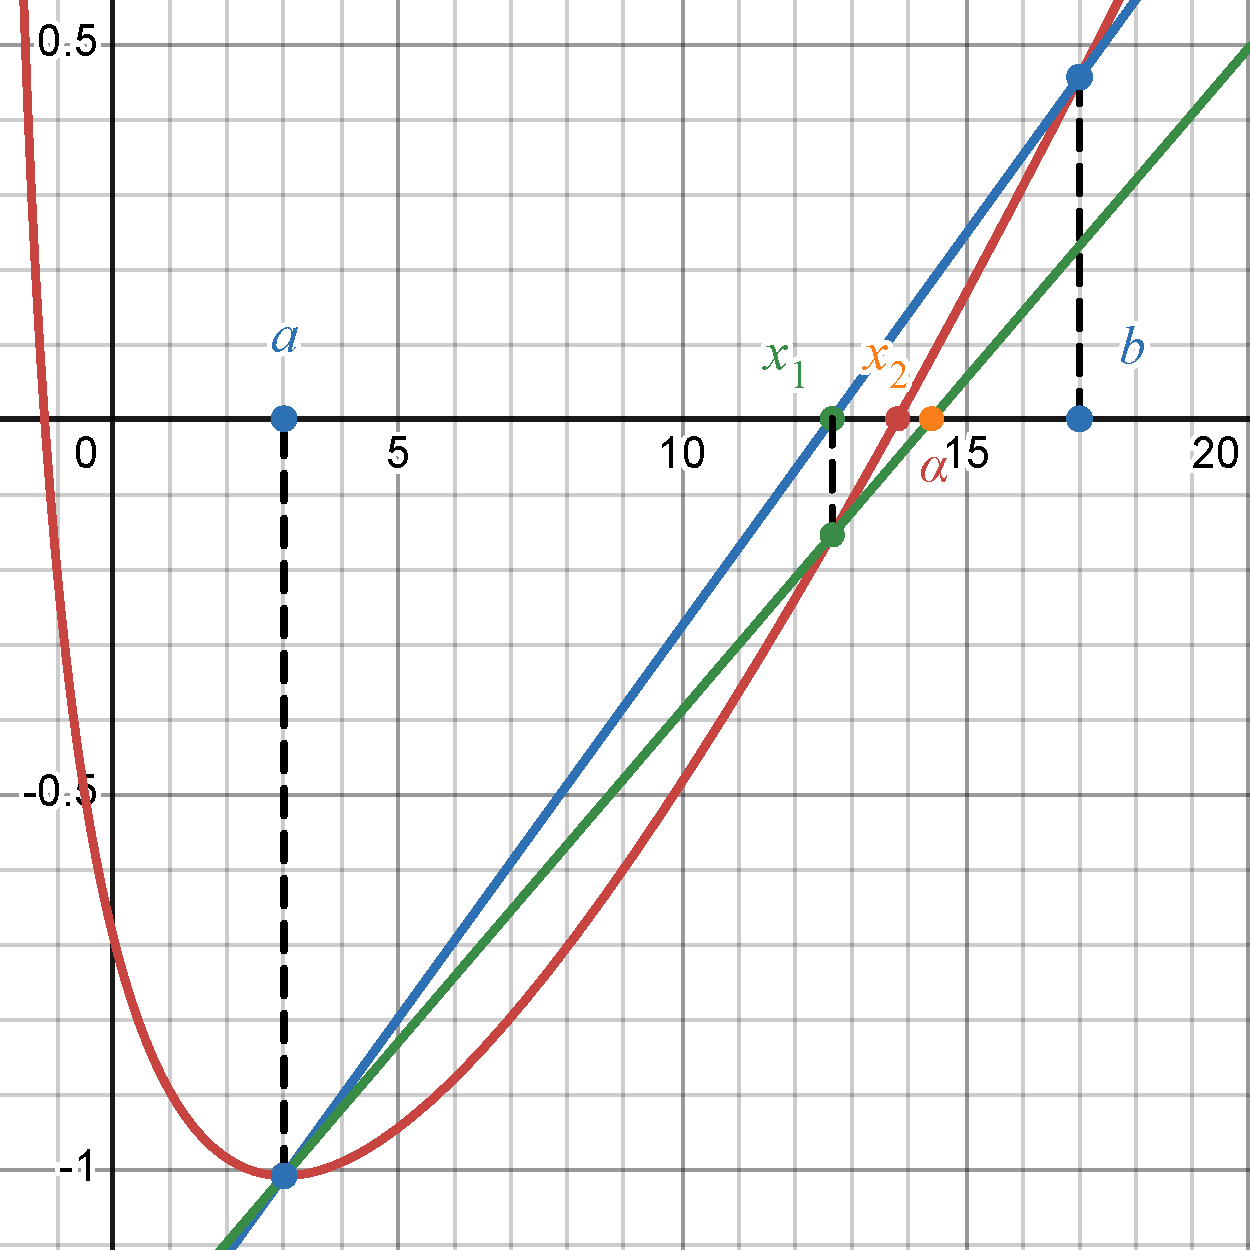
\includegraphics[width=0.69\textwidth]{../Diagrams/linear-interpolation.pdf}
        \caption{An illustration of linear interpolation \href{https://www.desmos.com/calculator/jp52nra5le}{(Desmos)}.}
        \label{fig:linear-interpolation}
        % The second and third lines are wrong! 
    \end{figure}
    \begin{figure}[H]
        \centering
        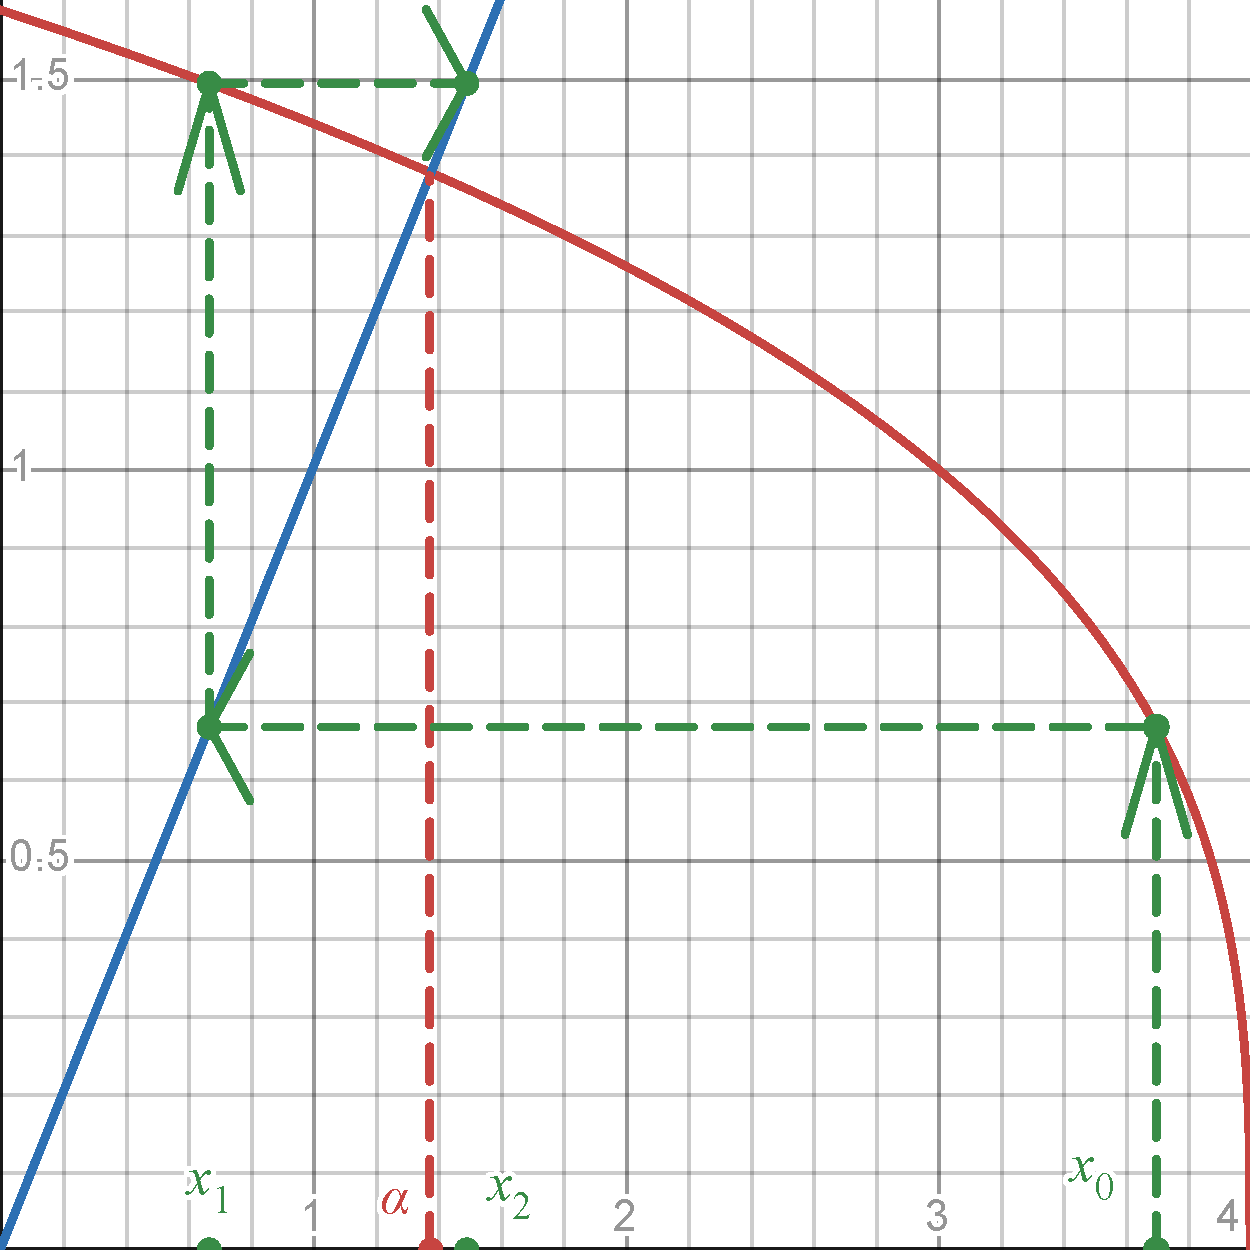
\includegraphics[width=0.69\textwidth]{../Diagrams/fixed-point-iteration/fixed-point-iteration-desmos.pdf}
        \caption{An illustration of fixed-point iteration \href{https://www.desmos.com/calculator/t9mnqtmhxw}{(Desmos)}.}
        \label{fig:fixed-point-iteration}
    \end{figure}
    % \begin{figure}[H]
    %     \centering
    %     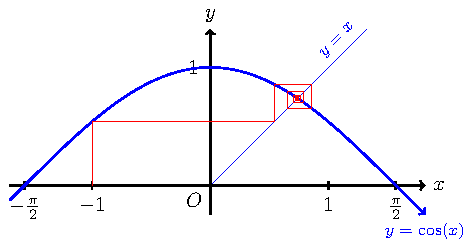
\includegraphics[width=\textwidth]{../Diagrams/fixed-point-iteration/fixed-point-iteration.pdf}
    %     \caption{An illustration of fixed-point iteration.}
    %     \label{fig:fixed-point-iteration}
    % \end{figure}
    \begin{figure}[H]
        \centering
        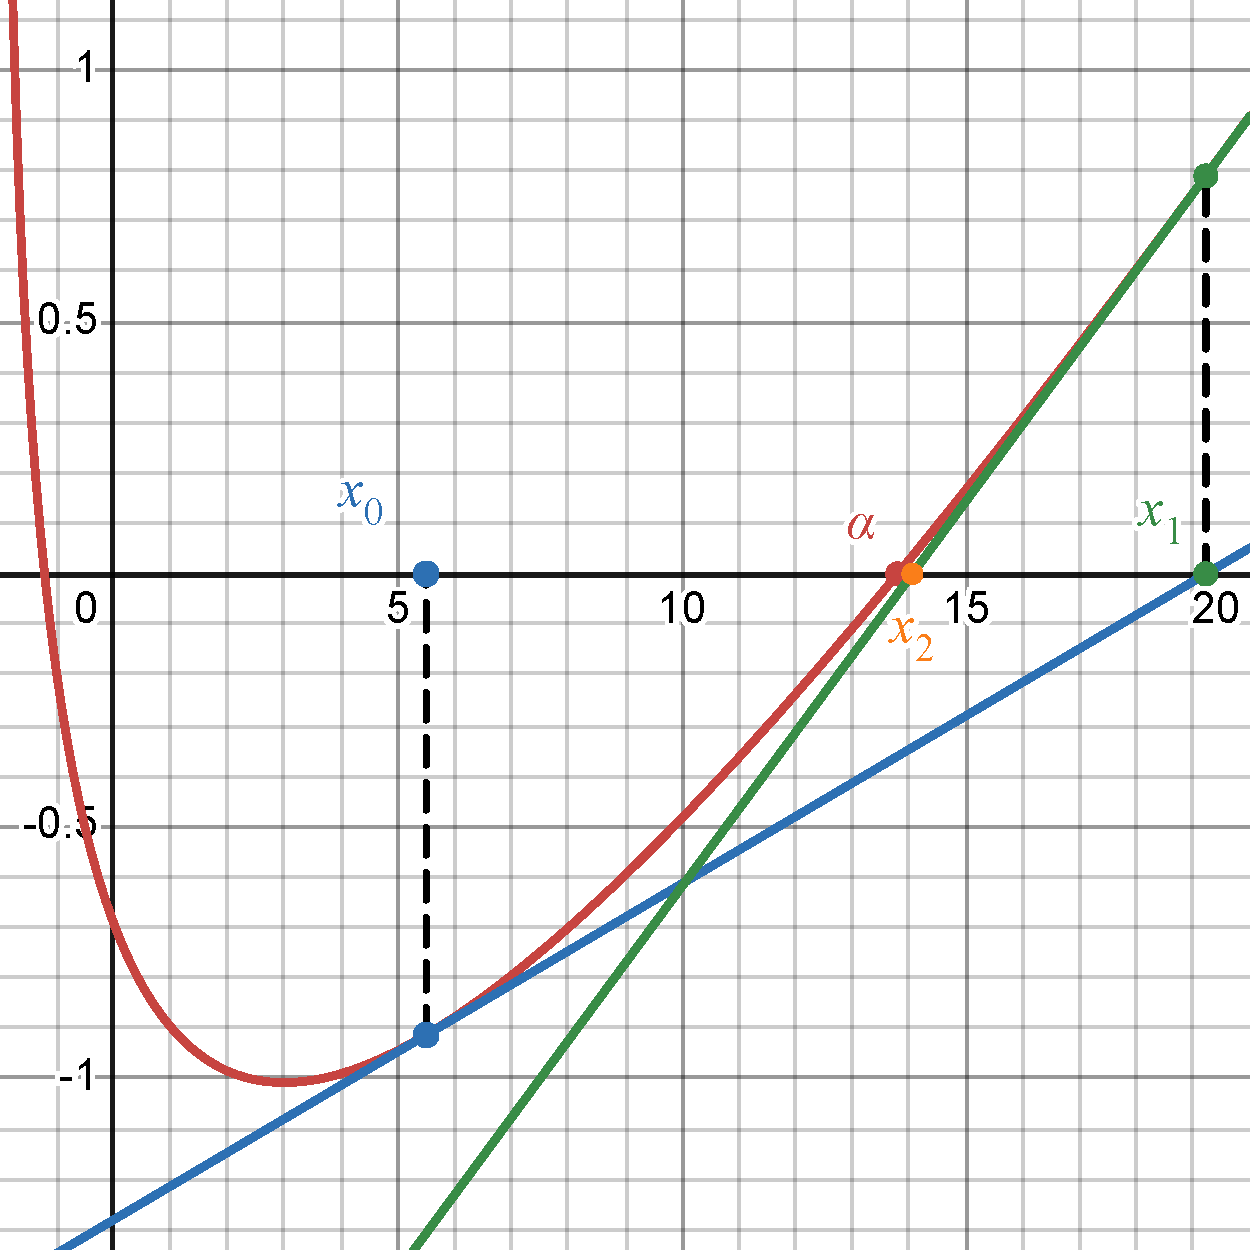
\includegraphics[width=0.69\textwidth]{../Diagrams/newton's-method.pdf}
        \caption{An illustration of Newton's Method \href{https://www.desmos.com/calculator/izkg4ynlfp}{(Desmos)}.}
        \label{fig:newton's-method}
    \end{figure}
    \begin{note}
        Perform \rule{1.5cm}{0.01mm} (e.g. linear interpolation) to obtain an approximation for \(\alpha\), correct to two decimal places. Justify whether this approximation is sufficiently accurate.

        \rule{20cm-137.0549pt}{0.05mm}

        Suppose our approximation is some \(a=1.00\), then we note the sign of \(f\) at \(a\pm 0.\highlight[yellow]{00}5\). (For an arbitrary number of s.f. or d.p., simply adjust the value \(0.\highlight[yellow]{00}5\) accordingly. E.g. for 3 d.p. we instead use \(0.\highlight[yellow]{000}5\)). Our working should look similar to the following:
        \begin{center}
            \parbox{0.9\textwidth}{
                Since \(f(0.995)=\rule{0.5cm}{0.01mm}<0\) and \(f(1.005)=\rule{0.5cm}{0.01mm}>0\), we conclude that \(1.00\) is a sufficiently accurate approximation, at 2 d.p..
            }
        \end{center}
    \end{note}
\end{document}